\documentclass{article}
\usepackage[utf8]{inputenc}
\usepackage[russian]{babel}
\usepackage{graphicx}
\usepackage{caption}
\usepackage{float}
\usepackage{hyperref}
\usepackage{xcolor}
\usepackage{amsmath}
\usepackage[unicode, pdftex]{hyperref}
\usepackage[left=2cm,right=2cm,
    top=2cm,bottom=2cm,bindingoffset=0cm]{geometry}
    
\graphicspath{{pictures/}}
\DeclareGraphicsExtensions{.pdf,.png,.jpg}
\definecolor{urlcolor}{HTML}{003bed}
\hypersetup{pdfstartview=FitH, linkcolor=linkcolor,urlcolor=urlcolor, colorlinks=true}
\begin{document}
    \begin{center}
        \hfill \break

        \LARGE{Математический анализ}\\
        \hfill \break
        \normalsize{Модуль 4\\
        \hfill \break
        2021 год\\
        \hfill \break
        «Кратные интегралы»}\\
        \hfill \break
        \hfill \break
        \hfill \break
        \hfill \break
    \end{center}

    \begin{flushright} Иванов Сергей, Иванов Алексей, Титов Даниил \end{flushright}
    \begin{flushright} M3104 \end{flushright}
    \vfill
    \bigskip
    \begin{center} Июнь 2021 \end{center}
    \begin{center} ИТМО \end{center}
    \thispagestyle{empty} % выключаем отображение номера для этой страницы
    \newpage
    \tableofcontents{}
    \vfill
    \bigskip
    \begin{flushright} \href{https://ru.overleaf.com/read/vdjmnbrygsdc}{Код отчёта на Overleaf (Latex)} \end{flushright}
    \newpage
    \section{Потенциал векторного поля}
        \subsection{Убедитесь, что поле потенциально. Найдите уравнения векторных линий. Изобразите Векторные линии на рисунке. Найдите потенциал поля при помощи криволинейного интеграла. Изобразите линии уровня потенциала (эквипотенциальные линии). Проиллюстрируйте ортогональность линий уровня и векторных линий. Зафиксируйте точки $A$ и $B$ на какой-либо векторной линии. Вычислите работу поля вдоль этой линии.}
            С формально-математической точки зрения, векторные поля задают векторными функциями:\\
            Для "плоского" случая - это векторная функция $\vec{F}(x, y) = P(x, y)\vec{i} + Q(x, y)\vec{j}$, которая различным точкам $M(x, y)$ плоскости $XOY$* ставит в соответствие несвободные векторы.\\
            *Далее по умолчанию считаем, что все дела происходят в декартовой системе координат\\\\
            С трёхмерным пространством аналогично\\
            $\vec{F}(x, y, z) = P(x, y, z)\vec{i} + Q(x, y, z)\vec{j} + R(x, y, z)\vec{k}$ - здесь каждой допустимой точке $M(x, y, z)$ пространства ставится в соответствие вектор $\vec{F}(x, y, z)$ с началом в данной точке.\\
            "Допустимость" определяется областями определения функций $P(x, y, z)\vec{i}$, $Q(x, y, z)\vec{j}$, $R(x, y, z)\vec{k}$, и если каждая из них определена на всех $x$, $y$ и $z$, то векторное поле будет задано во всём пространстве.\\\\
            Интегралььной кривой для поля $F(r)$ называется кривая $r = r(t)$, касательная к которой во всех точках кривой совпадает со значением поля:\\
            $\frac{dr}{dt} = F(r(t))$\\\\
            Примем:\\
            $P(x; y) = 1$\\
            $Q(x; y) = -\frac{1}{y^2}$\\
            $R(x; y) = 0 \Rightarrow $ можем рассматривать плоское поле\\
            Конечное уравнение поля\\
            $\vec{F}(x;y) = \vec{i}-\frac{1}{y^2}\vec{j}$\\
            $\vec{F} = (1;-\frac{1}{y^2};0)$\\
            \subsubsection{Проверка потенциальности поля}
                $] \frac{dP}{dy} = \frac{dQ}{dx} \Rightarrow$ поле потенциально \space; rot$\vec{F} = 0$\\
                $\frac{d(1)}{dy} = 0$, $\frac{d(-\frac{1}{y^2})}{dx} = 0$\\
                $0 = 0 \Rightarrow$ поле потенциально\\
            \subsubsection{Уравнение силовых (векторных) линий}
                Для нахождения силовых линий решим уравнение: $\frac{dx}{P} = \frac{dy}{Q}$\\
                $\begin{cases}
                    dz = 0 \Rightarrow z = c_2$ - семейство плоскостей $\parallel XOY\\
                    \frac{dx}{1} = \frac{dy}{-\frac{1}{y^2}}
                \end{cases}$\\
                $dx = -y^2dx$\\
                $\int\limits{dx} = -\int\limits{y^2dy}$\\
                $C^*$ - const\\
                $x = -\frac{y^3}{3} + C^* |*3$;\space $3*$const $=$ const\\
                $3x = -y^3 + 3C^*$; \space $3C^* =$ const $= C_1$\\
                $3x + y^3 = C_1$\\
                $y = \sqrt[3]{C_1 - 3x}$, $y \not = 0$\\
                Уравнение векторных линий:\\
                $\begin{cases}
                    3x + y^3 = C_1 \\
                    z = C_2
                \end{cases}$
            \subsubsection{Изображение векторных линий}
                Начнем с изображения линий на одной выбранной плоскости ($z = 0$)\\
                $y = \sqrt[3]{C_1 - 3x}$\\
                Исследуем этот график:\\\\
                1. Поиск точек пересечения с осями\\
                $y \not = 0$;\space $\sqrt[3]{C_1 - 3x} \not = 0$;\space $x \not = \frac{C_1}{3}$\\
                $x = 0$;\space $y = \sqrt[3]{C_1}$\\\\
                2. $y > 0$,\space $x > \frac{C_1}{3}$\\ 
                $y < 0$,\space $x < \frac{C_1}{3}$\\
                $D(y) \in R$ - исключая такие искы, при которых $y = 0$\\
                $E(y) \in R$\\
                3. Исследование производной\\
                $y' = (\sqrt[3]{C_1 - 3x})' = ((C_1 - 3x)^{\frac{1}{3}})' = \frac{1}{3}(C_1 - 3x)^{-\frac{2}{3}} * (-3) = -\frac{1}{\sqrt[3]{(C_1 - 3x)^2}}$\\
                $y' = 0$;\space $x \in \not 0$\\
                $y'$ не существует - $C_1 - 3x \not = 0$;\space $x = \frac{C_1}{3}$\\
                \begin{figure}[h!]
                    \center{\fbox{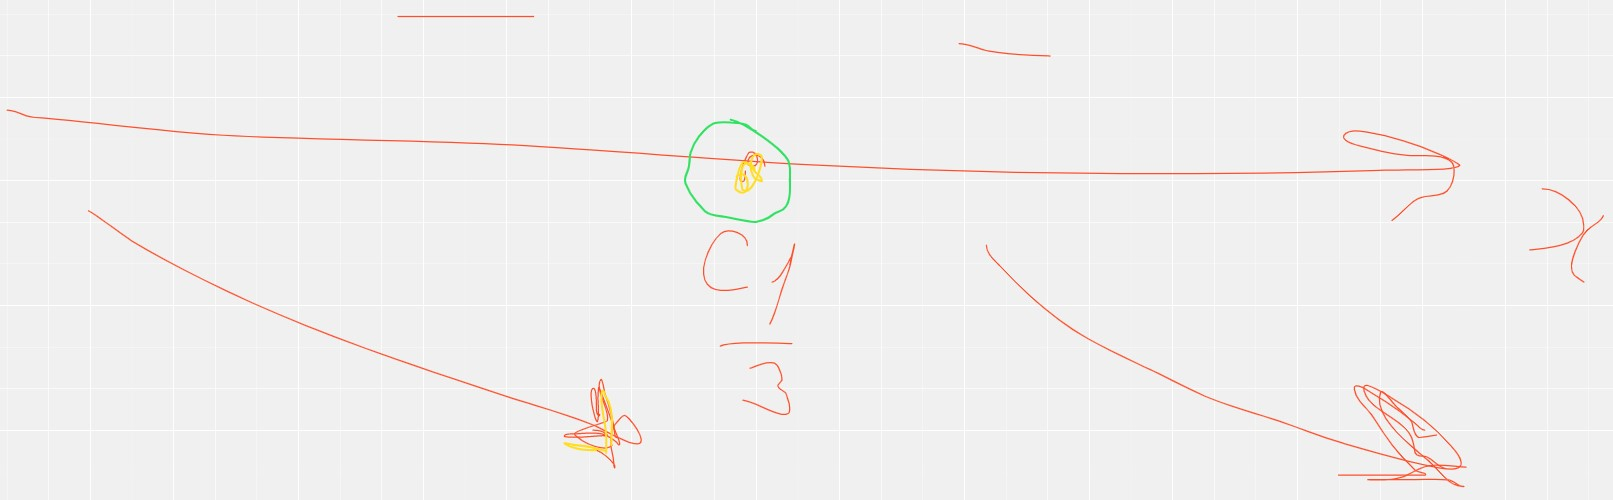
\includegraphics[scale=0.5]{image13}}}
                \end{figure}\\
                Получаем, что граф сильно зависит от $x = \frac{C_1}{3}$ - точка перегиба куба, получаем семейство движущихся корней с выколотым множеством точек, при которых $y = 0$\\
                \begin{figure}[h!]
                    \center{\fbox{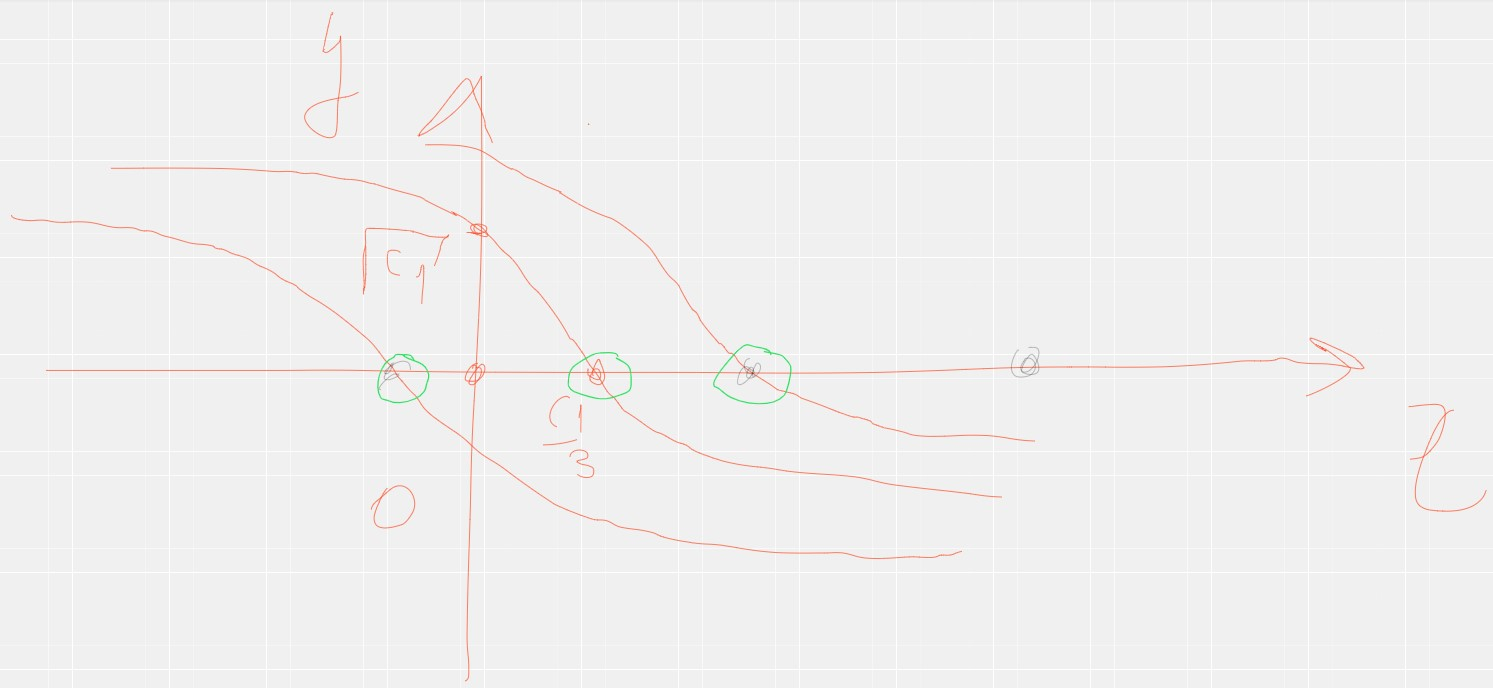
\includegraphics[scale=0.5]{image11}}}
                \end{figure}
                \newpage
                Если рисовать в 3-й форме:\\
                \begin{figure}[h!]
                    \center{\fbox{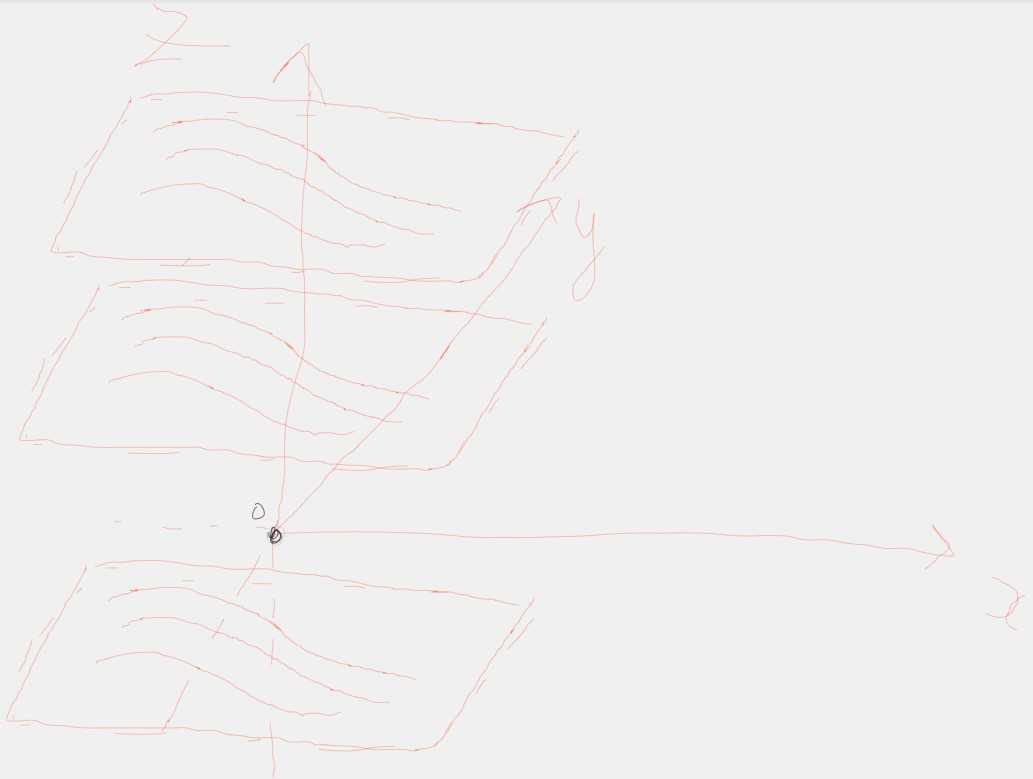
\includegraphics[scale=0.5]{image12}}}
                \end{figure}\\
                \subsubsection{Найдите потенциал поля при помощи криволинейного интеграла}
                Поиск потенциала\\
                $U(x, y, z) = \int\limits^x_{x_0}{F_x(x, y_0, z_0)dx} + \int\limits^y_{y_0}{F_y(x, y, z_0)dy} + \int\limits^z_{z_0}{F_z(x, y, z)dz} + C$\\
                Функции $F_x$ и $F_z$ непрерывны во всех точках пространства поля $\Rightarrow$ можем взять начальную точку $(0; y_0; 0)$\\
                $U(x, y, z) = \int\limits^x_0{1da} + \int\limits^y_{y_0}{-\frac{1}{b^2}db} + C = a |^x_0 - \int\limits^y_{y_0}{\frac{db}{b^2}} + C = x - 0 - (-\frac{1}{b} |^y_{y_0}) + C = x + \frac{1}{y} - \frac{1}{y_0} + C = x + \frac{1}{y} + C \leftarrow$ возьмём координату начальной точки $y_0 \rightarrow \infty \Rightarrow \frac{1}{y_0} \rightarrow 0 \Rightarrow$ можем пренебречь значением $\frac{1}{y_0}$\\\\
                \subsubsection{Изобразите линии уровня потенциала. Проиллюстрируйте ортогональность линий уровня и векторных линий}
                Чтобы линия была эквипотенциальной необходимо, чтобы вдоль этой линии (то есть для каждой ее точки) значение потенциала было постоянным\\
                $x + \frac{1}{y} = const$\\
                $\frac{1}{y} = \frac{const}{1}-x$\\
                $y = \frac{1}{const - x_0}$\\\\
                Из уравнения очевидно, что график функции - гипербола\\
                Аналогично построим эквипотенциальные линии при нескольких константных значениях правой части равенства, вместе с векторными для демонстрации их ортогональности
                \begin{figure}[h!]
                    \center{\fbox{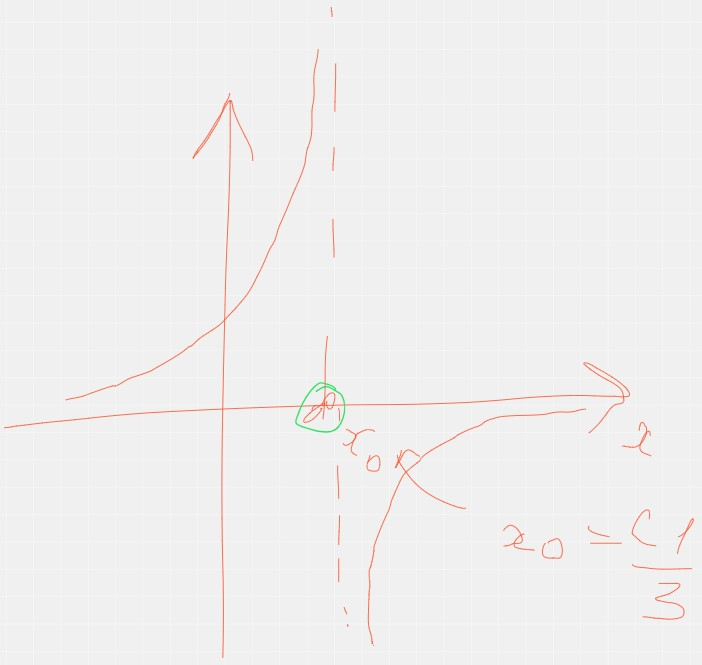
\includegraphics[scale=0.5]{image14}}}
                \end{figure}\\
                \begin{figure}[h!]
                    \center{\fbox{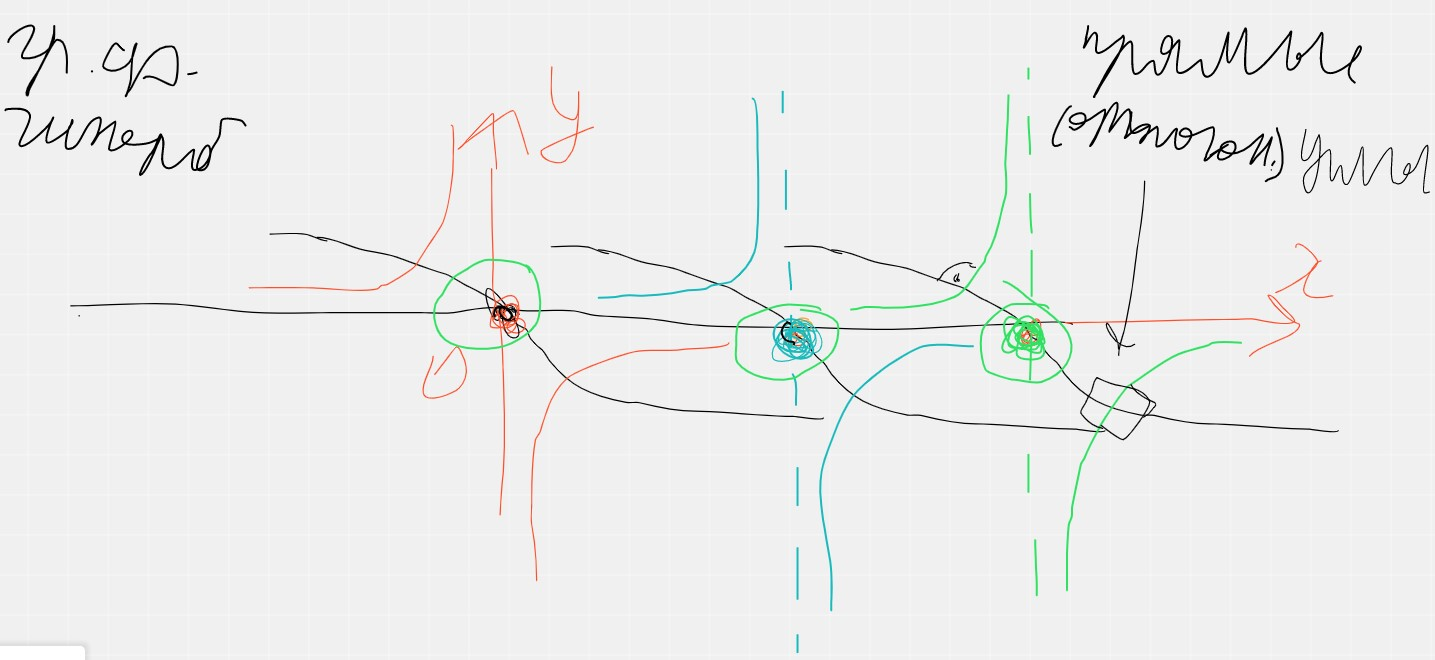
\includegraphics[scale=0.5]{image15}}}
                \end{figure}
                \newpage
                \begin{figure}[h!]
                    \center{\fbox{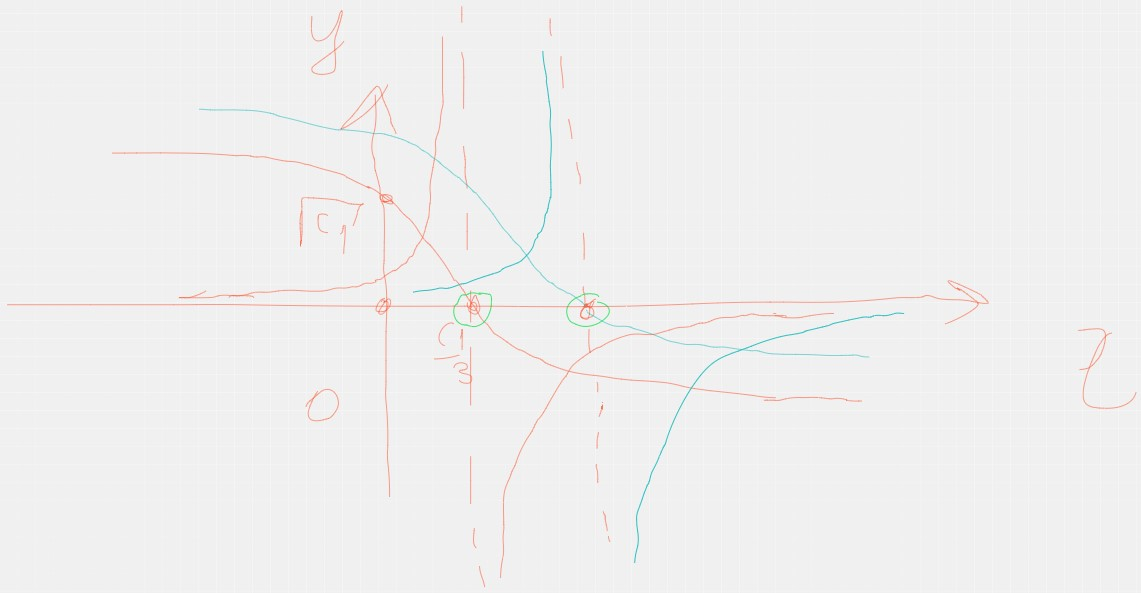
\includegraphics[scale=0.5]{image16}}}
                \end{figure}\\
                \subsubsection{Зафиксируйте точки A и B на какой-либо векторной линии. Вычислите работу поля вдоль этой линии}
                Берём точку $B(0, 1, 0)$, а так как точка $B(0, 1, 0)$ или $(0, 1) \in y \Rightarrow 1 = \sqrt[3]{C_1 - 0} \Rightarrow C_1 = 1$\\
                $y = \sqrt[3]{C_1 - 3x}$\\
                $y_{рассм} = \sqrt[3]{1 - 3x}$\\
                $1 - 3x = t^3$\\
                $x = \frac{1 - t^3}{3} \in z$, где $t = 4$\\
                $x_1 = \frac{1-64}{3} = -21$\\
                $y_1(x) = \sqrt[3]{1+63} = \sqrt[3]{64} = 4$\\
                Вторая точка $A(-21, 4, 0)$\\
                \begin{figure}[h!]
                    \center{\fbox{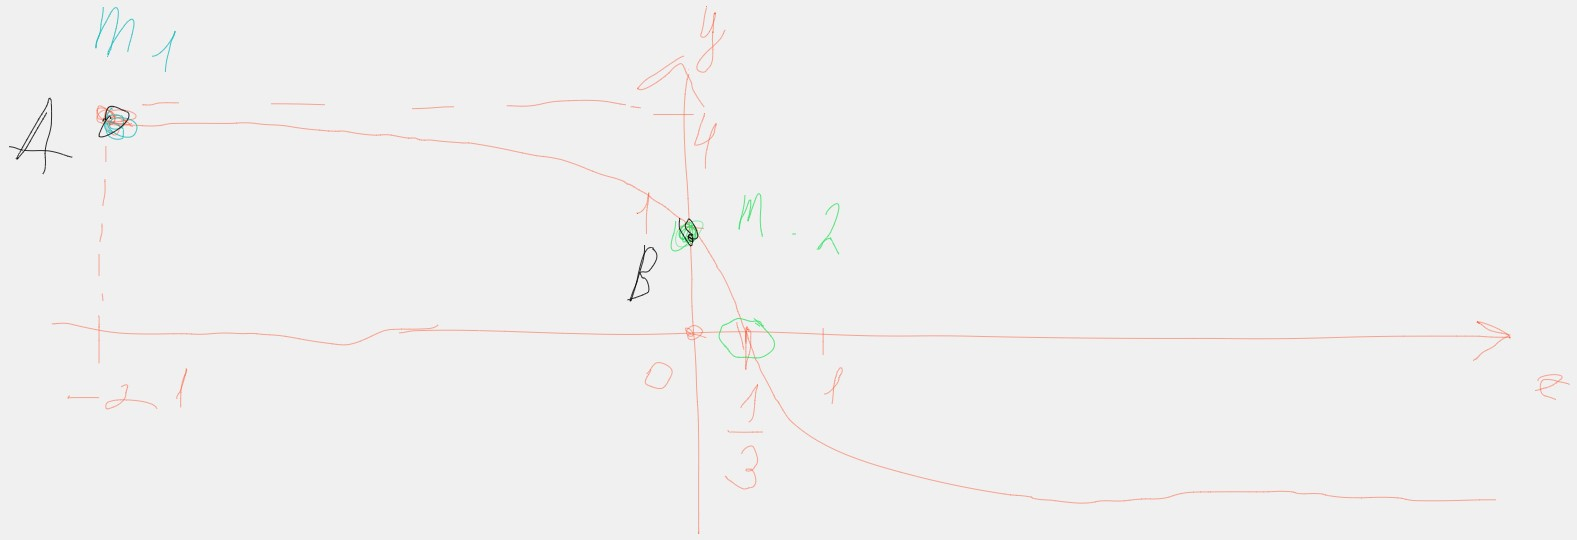
\includegraphics[scale=0.5]{image17}}}
                \end{figure}\\
                $y = \sqrt[3]{1 - 3x}$\\
                $dy = -\frac{1}{(1 - 3x)^{\frac{2}{3}}}dx$\\
                Работа между двумя точкам $(-21, 4, 0)$ и $(0, 1, 0)$ по кривой $y = \sqrt[3]{1 - 3x}$\\
                Будем интегрировать по $dx \Rightarrow$ пределы интегрирования $-21 \le x \le 0$\\
                $A = \int\limits_L{1dx} - \frac{1}{y^2}dy = \int\limits^0_{-21}{dx} - \frac{1}{(1 - 3x)^{\frac{2}{3}}} * (-\frac{1}{(1 - 3x)^{\frac{2}{3}}}dx) = \int\limits^0_{-21}{1 + \frac{1}{(1-3x)^{\frac{4}{3}}dx}} = x + \frac{1}{\sqrt[3]{1 - 3x}} |^0_{-21} = 1 - (-21 + \frac{1}{4}) = 22 - \frac{1}{4} = \frac{87}{4}$\\
                $U = x + \frac{1}{y}$\\
                $U(B) = 0 + 1 = 1$\\
                $U(A) = -21 + \frac{1}{4}$\\
                $A = U(B) - U(A) = 1 - (-21 + \frac{1}{4}) = 22 - \frac{1}{4} = \frac{87}{4}$\\
                Значения, полученные при вычислении работы вдоль выбранной векторной линии с помощью криволинейного интеграла и разности потенциалов одинаковы и численно равны $\frac{87}{4}$
                \subsubsection{Выводы}
                1. Доказали, что наше изначальное поле потенциально, поскольку ротор поля равен 0\\
                2. Построили графики и нашли уравнение векторных линий. Уравнения:\\
                $\begin{cases}
                    3x + y^3 = C_1 \\
                    z = C_2
                \end{cases}$\\\\
                Вид графика - множество кубических корней\\
                3. При помощи криволинейного интеграла нашли функцию потенциала поля $U(x, y, z) = x + \frac{1}{y} + C$\\
                4. Нашли уравнения и построили графики эквипотенциальных линий. Из уравнения графика получили, что график линии - гипербола. Соотнесли графики векторных линий и эквипотенциальных линий. По графикам и по свойствам функций продемонстрировали, что данные линии ортогональны\\
                5. Произвольно выбрали 2 точки, принадлежащие произвольной векторной линии, посчитали работу поля между этими точками при помощи криволинейного интеграла и разности потенциалов. Получили одинаковые значения, это ещё раз доказывает потенциальность (консервативность) силы поля
                \newpage
    \section{Поток векторного поля}
        \subsection{Дано тело $Т$, ограниченное следующими поверхностями:\\
        $z + \sqrt{4 - x^2 - y^2} = 0, 2(z + 1) - \sqrt{x^2 + y^2} = 0$\\
        На рисунке представлено сечение тела $Т$ координатной плоскостью $Oyz$.\\
        Изобразите тело $Т$ на графике в пространстве.\\
        Вычислите поток поля $\vec{a} = (\sin{yz})\vec{i} + (xe^{2x^{2}} + e^{z})\vec{j} - z\vec{k}$ через боковую поверхность тела $T$, образованную вращением дуги $BCD$ вокруг оси $Oz$, в направлении внешней нормали поверхности тела $Т$.}
        \begin{figure}[h!]
            \fbox{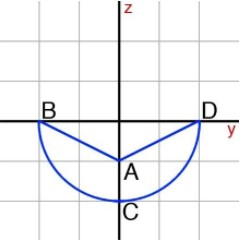
\includegraphics[scale=0.5]{image23}}
        \end{figure}\\
        \href{https://www.geogebra.org/3d/vgwdzge5}{Ссылка на geogebra.org, где был построен график}\\
        a)\\
        \begin{figure}[h!]
            \center{\fbox{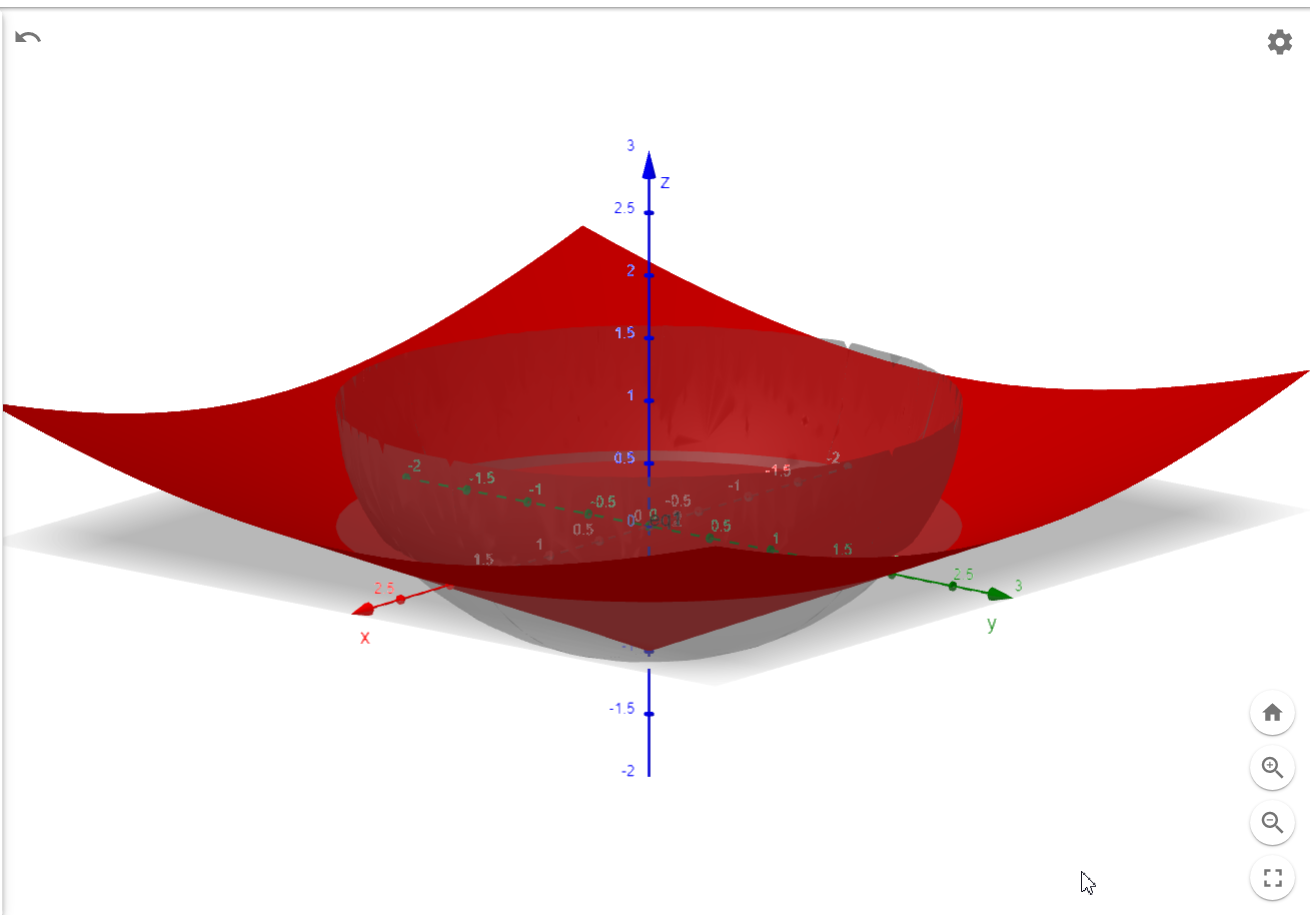
\includegraphics[scale=0.3]{image.png}}}
        \end{figure}
        \newpage
        \begin{figure}[h!]
            \center{\fbox{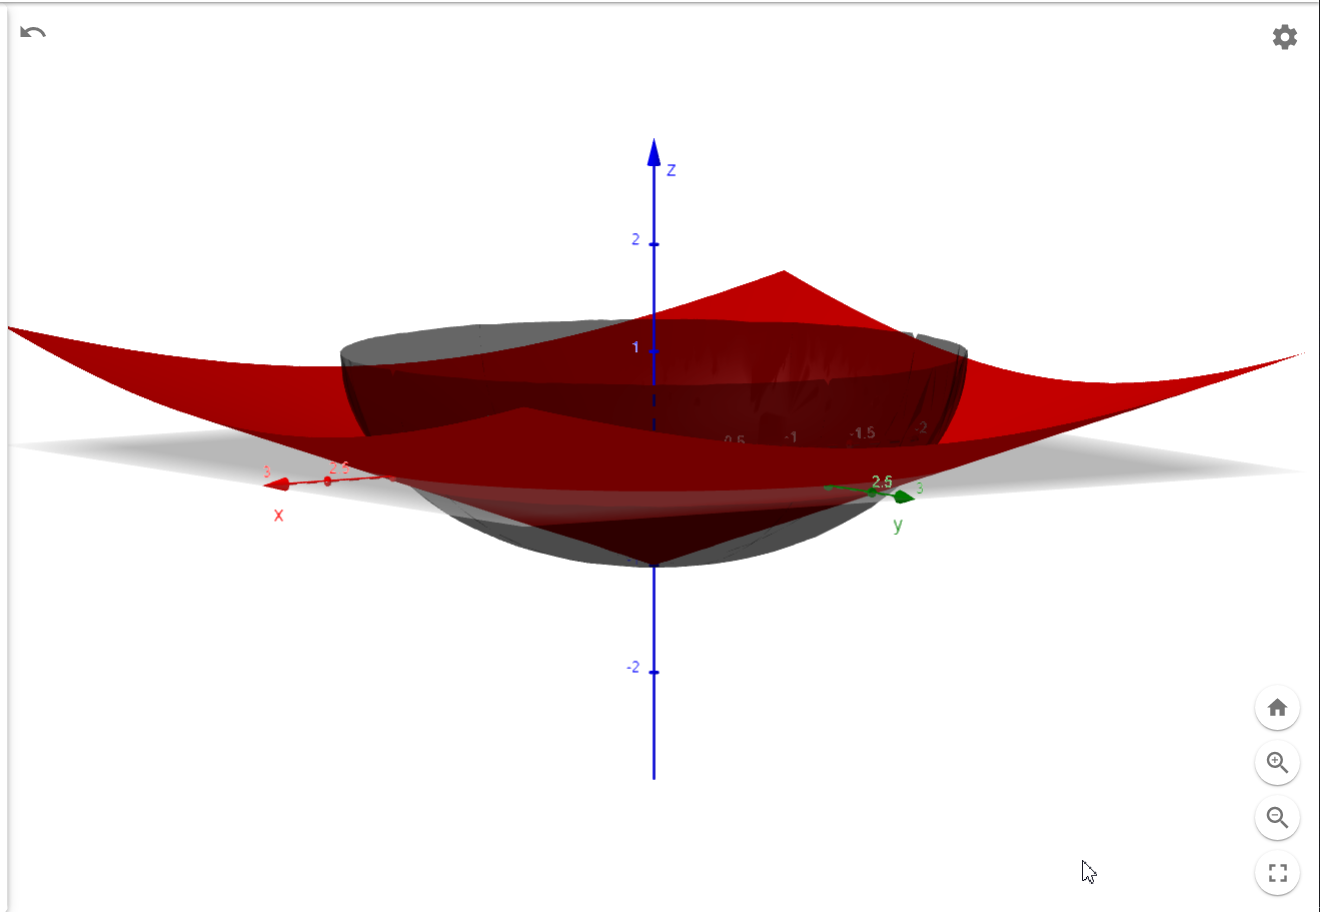
\includegraphics[scale=0.3]{image2.png}}}
        \end{figure}\\\\
        b)\\
        $\Pi = \int\limits{\int\limits_V{\int\limits{div\vec{a}dV}}}$\\
        $div\vec{a} = \frac{\partial(\sin{yz})}{\partial x} + \frac{\partial(xe^{2x^2} + e^z)}{\partial y} - \frac{\partial z}{\partial z} = 0 + 0 - 1 = -1$\\
        $x = \rho\cos{\varphi}\sin{\Theta}$\\
        $y = \rho\sin{\varphi}\sin{\Theta}$\\
        $z = \rho\cos{\Theta}$\\
        $dxdydz = \rho^2\sin{\Theta}d\rho d\varphi d\Theta$\\\\
        $\Pi_1 = -1 \int\limits{\int\limits_V{\int\limits{dV}}} = -\int\limits{\int\limits_V{\int\limits{dxdydz}}} = -\int\limits{\int\limits_V{\int\limits{\rho^2\sin{\Theta}d\rho d\varphi d\Theta}}} = -\int\limits^2_0{\rho^2d\rho \int\limits^{\pi}_{\frac{\pi}{2}}\sin{\Theta}d\Theta \int\limits^{2\pi}_{0}d\varphi} = -(\frac{\rho^3}{3} |^2_0 *(-\cos{\Theta} |^{\pi}_{\frac{\pi}{2}}) * (\varphi |^{2\pi}_0)) = - (\frac{8}{3}*(-(-1 - 0)*(2\pi - 0))) = -\frac{16\pi}{3}$\\
        $\Pi_2$ - через круг $x^2 + y^2 = 4$\\
        $\vec{n} = (0, 0, 1)$\\
        $\Pi_2 = \int\limits_S{\int\limits{(\vec{a}, \vec{n})dS}} = \int\limits_S{\int\limits{-zdS}} = \int\limits^2_{-2}{dx \int\limits^{\sqrt{4 - x^2}}_{-\sqrt{4 - x^2}}{-zdy}} = -2z\int\limits^2_{-2}{\sqrt{4 - x^2}dx} = -4\pi z$\\
        Для $z = 0: \Pi_2 = 0$\\\\
        Ответ: $\Pi = \Pi_1 - \Pi_2 = -\frac{16\pi}{3}$
\end{document}